\chapter{Firmenverwaltung}
\label{Firmenverwaltung}
Die Firmenverwaltung ist im FAS �ber den Men�punkt Extras->Firmenverwaltung erreichbar.
�ber diese Firmenverwaltung werden alle Firmen verwaltet die im FH-Complete zu Verf�gung gestellt werden.
Zum Beispiel f�r Lehrauftr�ge, Projektarbeiten/Berufspraktika, Schulen f�r das PreInterressenten-Tool oder auch f�r die Erhalter Standorte.\\
�ber das Suchfeld k�nnen Sie nach einer bestimmten Firma suchen. Zus�tzlich kann die Suche nach dem Typ der Firma eingeschr�nkt werden.
Durch einen klick auf die ID oder den Namen der Firma werden die Details angezeigt.
\section{Anlegen einer neuen Firma}
Zum Anlegen einer neuen Firma klicken Sie auf "Neue Firma anlegen". F�llen Sie anschliesen die Daten aus und dr�cken Sie auf  speichern.
\section{Standorte}
Eine Firma kann �ber mehrere Standorte verf�gen. �ber den Punkt "Neuanlage" k�nnen zus�tzliche Standorte angelegt werden.
Mit einem klick auf die Kurzbezeichnung des Standortes kann dieser editiert werden. Hier k�nnen weiter Informationen eingetragen werden wie etwa Adresse, Ansprechpartner oder zus�tzliche Kontaktdaten wie Telefon oder E-Mail.
\begin{figure}
	\centering
	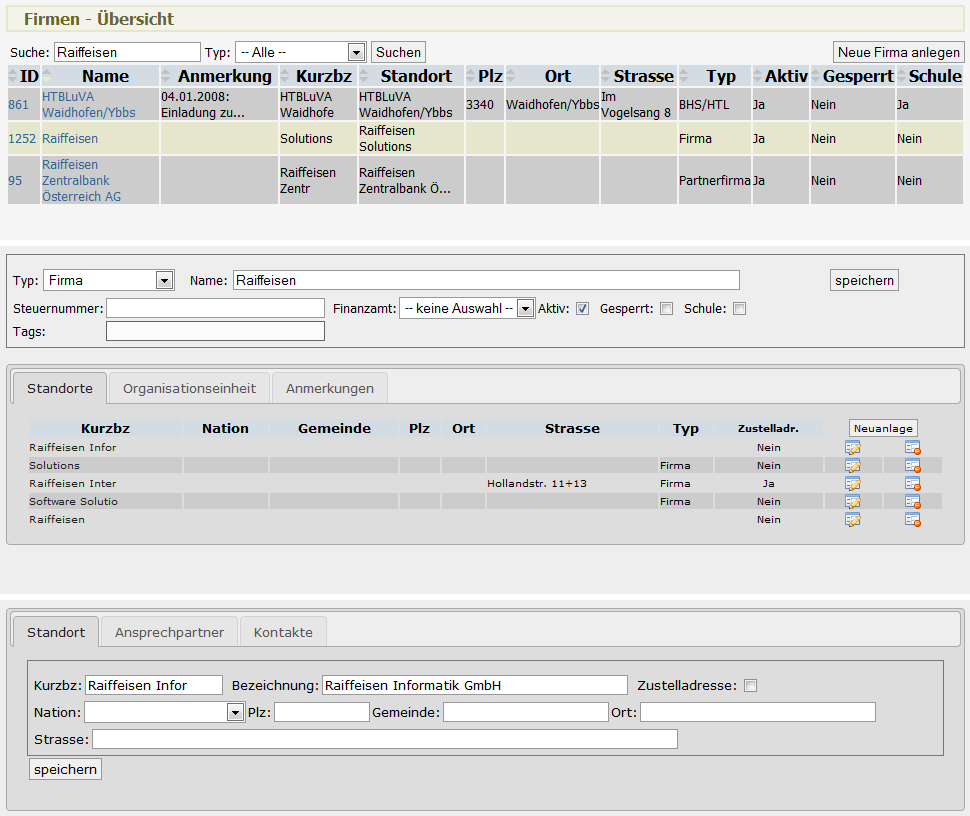
\includegraphics[width=1\textwidth]{FASo_Firmenverwaltung.png}
	\caption{Firmenverwaltung}
	\label{Firmenverwaltung}
\end{figure}
\section{Organisationseinheit}
�ber den Karteireiter Organsationseinheit, kann die Firma einem Studiengang, einem Institut oder einer Abteilung zugeordnet werden.
Diese Zuteilung hat derzeit noch keine Auswirkung.
\section{Tags}
Sie k�nnen Firmen mit Tags versehen. Tags sind kurze Schlagworte zur Kategorisierung. Um Tags zuzuordnen tippen Sie es in das Feld Tags. Wenn Sie mehrere Tags auf einmal zuweisen m�chten, trennen Sie diese mittels Strichpunkt.\\
�ber die Suche k�nnen Sie nach Firmen suchen, denen ein bestimmter Tag zugewiesen ist. Tragen Sie dazu einfach den Tag-Namen in das Suchfeld ein.
Um einen Tag wieder zu entfernen klicken Sie auf das Symbol rechts neben dem zu l�schenden Tag.